\documentclass[12pt]{article}

\usepackage[a4paper, margin=1in]{geometry}
\usepackage{graphicx}
\usepackage[absolute, overlay]{textpos}
\usepackage{fancyhdr}
\usepackage{siunitx}
\usepackage{tikz}
\usepackage{pgfplots}
\usetikzlibrary{decorations.pathmorphing}
\usetikzlibrary{math}
\usetikzlibrary{calc}

\pgfplotsset{compat=1.18}

\pagestyle{fancy} %for footers

\newcommand{\customsubject}{}   
\newcommand{\customtitle}{}

\newcounter{questionpartcounter}                  %Setup for question part counter for a,b,c listing
\renewcommand{\thequestionpartcounter}
{\alph{questionpartcounter}}

\newcounter{questionpartpartcounter}                  %Setup for question part  partcounter for a,b,c listing
\renewcommand{\thequestionpartpartcounter}
{\roman{questionpartcounter}}

\pagestyle{fancy} %for footers
\renewcommand{\headrulewidth}{0pt}
\fancyhf{}
\fancyfoot[R]{\thepage}

\newenvironment{worksheet}[2]
{
    
    \global\renewcommand{\customtitle}{#1}
    \global\renewcommand{\customsubject}{#2}


    \begin{textblock*}{5cm}(0.4cm,0.4cm)
   
\includegraphics[width=4cm]{include/figures/bmdwlogo}
\end{textblock*}

    \vspace*{-1cm}
    
    {\large\textbf{\begin{center}\customtitle\end{center}}}

    \begin{center}\customsubject\end{center}
    
    \vspace{0.3cm}
    
    \hspace*{-1.5cm}\textbf{Name:\ \rule{4cm}{0.4pt}}\; 
    \textbf{Student \#: \ \rule{3cm}{0.4pt}}\;
    \textbf{Student Email \#: \ \rule{1.53cm}{0.4pt}}

    \vspace{0.5cm}

    
    \begin{enumerate}
}
{
    \end{enumerate}
   % \begin{textblock*}{10cm}(1cm, 28cm) {\footnotesize \scriptsize \customsubject}
    
%\end{textblock*}
}



\newcommand{\question}[2][1cm]{%
    \item
    \setcounter{questionpartcounter}{0}
    \setcounter{questionpartpartcounter}{0}
    {#2}
    \vspace{#1}
}

\newcommand{\questionpart}[2][1cm]{%
    \setcounter{questionpartpartcounter}{0}
    \stepcounter{questionpartcounter}
    (\thequestionpartcounter)~#2
    \vspace{#1}
}

\newcommand{\questionpartpart}[2][1cm]{%
      \stepcounter{questionpartpartcounter}
      \thequestionpartpartcounter.~#2
      \vspace{#1}
}

\newcommand{\operation}[1]{%
{\large $
#1
$}
}



\begin{document}

\begin{worksheet}{Physics Worksheet}{Fluid Mechanics}

\question[0cm]{All of these shapes surround the same source}

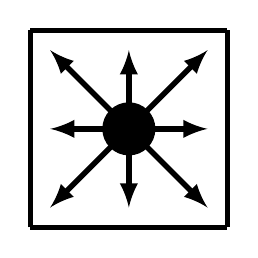
\begin{tikzpicture}
\draw[-latex,line width = 2pt] (0,0) -- (0,1);
\draw[-latex,line width = 2pt] (0,0) -- (1,1);
\draw[-latex,line width = 2pt] (0,0) -- (1,0);
\draw[-latex,line width = 2pt] (0,0) -- (1,-1);
\draw[-latex,line width = 2pt] (0,0) -- (-1,-1);
\draw[-latex,line width = 2pt] (0,0) -- (0,-1);
\draw[-latex,line width = 2pt] (0,0) -- (-1,1);
\draw[-latex,line width = 2pt] (0,0) -- (-1,0);
\draw[fill=black] (0,0) circle (0.33cm);

\draw[line width = 2pt] (-1.25,-1.25) -- (-1.25,1.25);
\draw[line width = 2pt] (-1.25,1.25) -- (1.25,1.25);
\draw[line width = 2pt] (1.25,1.25) -- (1.25,-1.25);
\draw[line width = 2pt] (-1.25,-1.25) -- (1.25,-1.25);

\end{tikzpicture}
\hspace{1cm}
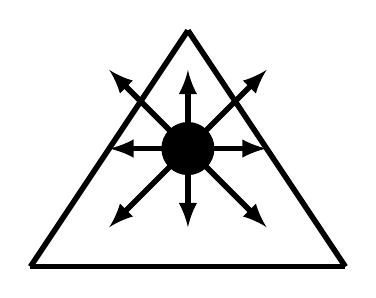
\begin{tikzpicture}
\draw[-latex,line width = 2pt] (0,0) -- (0,1);
\draw[-latex,line width = 2pt] (0,0) -- (1,1);
\draw[-latex,line width = 2pt] (0,0) -- (1,0);
\draw[-latex,line width = 2pt] (0,0) -- (1,-1);
\draw[-latex,line width = 2pt] (0,0) -- (-1,-1);
\draw[-latex,line width = 2pt] (0,0) -- (0,-1);
\draw[-latex,line width = 2pt] (0,0) -- (-1,1);
\draw[-latex,line width = 2pt] (0,0) -- (-1,0);
\draw[fill=black] (0,0) circle (0.33cm);

\draw[line width = 2pt] (-2,-1.5) -- (2,-1.5);
\draw[line width = 2pt] (-2,-1.5) -- (0,1.5);
\draw[line width = 2pt] (2,-1.5) -- (0,1.5);
\end{tikzpicture}
\hspace{1cm}
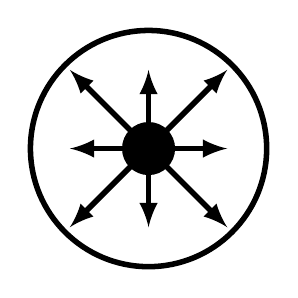
\begin{tikzpicture}
\draw[-latex,line width = 2pt] (0,0) -- (0,1);
\draw[-latex,line width = 2pt] (0,0) -- (1,1);
\draw[-latex,line width = 2pt] (0,0) -- (1,0);
\draw[-latex,line width = 2pt] (0,0) -- (1,-1);
\draw[-latex,line width = 2pt] (0,0) -- (-1,-1);
\draw[-latex,line width = 2pt] (0,0) -- (0,-1);
\draw[-latex,line width = 2pt] (0,0) -- (-1,1);
\draw[-latex,line width = 2pt] (0,0) -- (-1,0);
\draw[fill=black] (0,0) circle (0.33cm);

\draw[line width = 2pt] (0,0) circle (1.5cm);
\end{tikzpicture}


\questionpart[4cm]{Which of these shapes will report the highest flux? Explain}

\questionpart[4cm]{Which of these shapes would make the process of calculating the flux easiest?}

\question[0cm]{Consider an infinite wire carying a net positive charge}

\questionpart[0cm]{Draw a diagram of the wire and the theoretical field lines coming from it from a front, and a top down view}

\newpage

\questionpart[5cm]{What Guassian shape would make it easiest to calculate the flux coming from the wire?}

\questionpart[5cm]{Consider now a finite wire carrying a net positive charge. Why would calculating the flux coming from a finite wire more difficult that an infinire wire?}


\question[3cm]{What is the net flux coming out of an electric diapole?}








\end{worksheet}


\end{document}